The reported full-strategy pilot snapshot contains 100 completed independent markets (0 requested snapshot markets remain incomplete). Each has 500 stocks, 100 signals, one training block and 14 out-of-sample blocks of 252 days. Independent arithmetic replay covers 100 of these completed markets. These are pilot observations; the separate 500-market final study is not asserted to be complete. Earlier baseline and fixed-reference markets, and later markets outside the specified snapshot, are not added to this count.

\begin{table}[H]\centering\small

\begin{tabular}{lrrrr}

\toprule

Method & $h\bar U$ (MC SE) & Mean wealth & Inactive & Mean moves \\

\midrule

All Signals & 0.04429 (0.00113) & 1.889 & 0.000 & 0.00 \\

Greedy & 0.05166 (0.00074) & 2.083 & 0.071 & 6.47 \\

HAC & 0.05100 (0.00075) & 2.064 & 0.071 & 2.87 \\

Catoni & 0.00000 (0.00000) & 1.000 & 1.000 & 0.00 \\

Tail & 0.01104 (0.00043) & 1.170 & 0.821 & 0.99 \\

Oracle & 0.05844 (0.00050) & 2.282 & 0.000 & 0.00 \\

\bottomrule\end{tabular}

\caption{Full-strategy pilot means. Utility is daily utility rescaled by $h=252$, not an annual certainty equivalent. MC SE uses independent markets. Wealth includes waiting in cash and all modeled actual fund costs. Moves include terminal choices, which create no post-choice fund return.}\end{table}

Tail makes 99 choices (ENTRY: 99, PARK: 0, REVIVE: 0, SWAP: 0), of which 99 are executed before the horizon. Its mean inactive fraction is 0.821. Successful initial certification therefore must be assessed alongside the returns foregone during waiting. The lifecycle counts delimit what this pilot can say about parking and revival.

\begin{table}[H]\centering\small

\begin{tabular}{lrrr}

\toprule

Method & Eligible stable events & Criterion within year & Selected within year \\

\midrule

Greedy & 7515 & 6435 & 368 \\

HAC & 5962 & 3788 & 199 \\

Catoni & 4787 & 0 & 0 \\

Tail & 4760 & 0 & 0 \\

\bottomrule\end{tabular}

\caption{Response-independent stable-event cohorts with a full year of calendar follow-up. Each row has its own endogenous reference policies and event population; raw counts do not identify causal cross-method detection performance. Dependent events are not treated as independent replications.}\end{table}

\begin{table}[H]\centering\small

\begin{tabular}{lrrrr}

\toprule

Method & Executed & Positive gain & Mean gain (bp) & Entry cost (bp) \\

\midrule

Greedy & 620 & 0.140 & -0.712 & 1.190 \\

HAC & 285 & 0.305 & -0.256 & 1.291 \\

Tail & 99 & 1.000 & 0.931 & 1.500 \\

\bottomrule\end{tabular}

\caption{Evaluator-only next-period gains from the actual previous allocation, including modeled transition costs. These descriptive outcomes concern executed decisions, exclude terminal certifications, and are not quantities certified by a historical episode rejection.}\end{table}

\begin{figure}[H]\centering

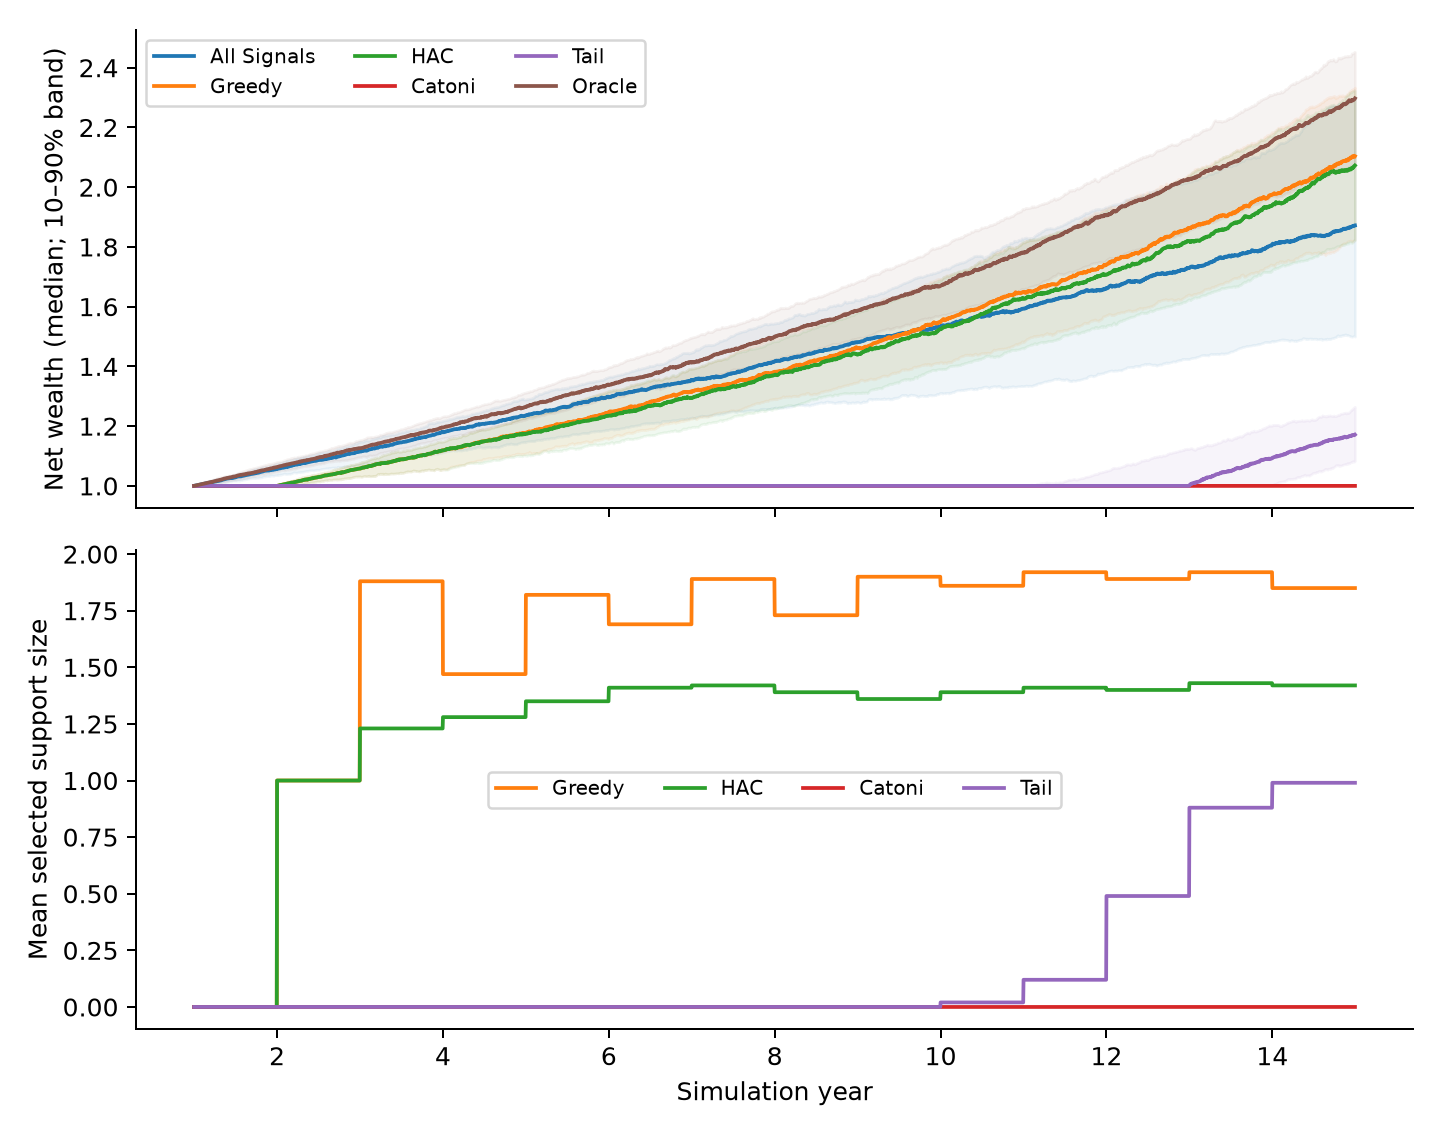
\includegraphics[width=.96\linewidth]{figures/full_strategy_paths.png}

\caption{Actual net wealth and selected support size in the completed full-strategy pilot. Wealth bands are the 10th and 90th market percentiles; they are descriptive quantiles, not confidence intervals.}

\end{figure}

\begin{figure}[H]\centering

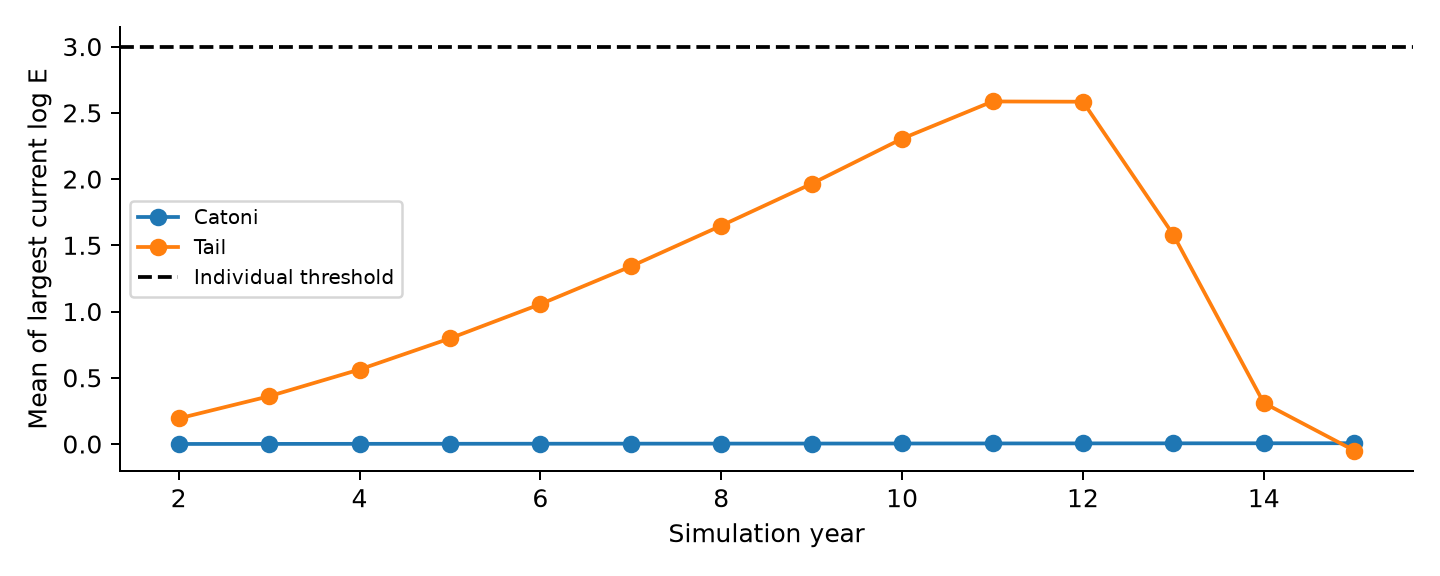
\includegraphics[width=.96\linewidth]{figures/full_strategy_evidence.png}

\caption{Mean across completed markets of the largest currently open annual log capital. Closed comparisons are not carried forward. The dashed line is the individual threshold; it does not protect the entire search.}

\end{figure}

Paired Tail-minus-reference differences in $h\bar U$ (95\% Student MC intervals) are All Signals: -0.03325 [-0.03560, -0.03089]; Greedy: -0.04062 [-0.04187, -0.03938]. These exploratory intervals use independent paired markets and are unadjusted across comparisons; they do not give guarantees for a new financial law. The reproducibility tables retain every benchmark contrast.

All Signals permits every candidate but does not hold all of them: its mean number of positions exceeding $10^{-6}$ in absolute sleeve weight is 4.54. This descriptive count is computed after the run and changes no allocation or test. The optimizer already produces a sparse portfolio, so it is a substantive baseline for the value of an additional statistical support filter. No fixed per-signal research cost is charged in this design.

Catoni executes a move in 0 of 100 markets (Wilson 95\% interval for the market-level fraction [0.000, 0.037]). A zero observed fraction does not establish zero probability of future entry.
